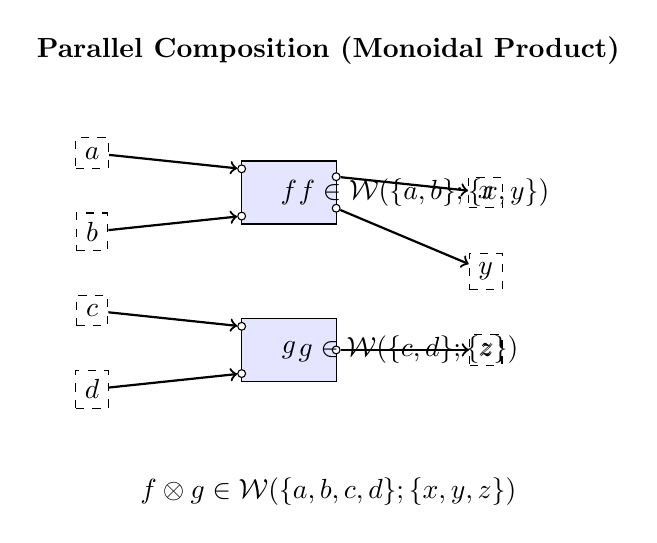
\begin{tikzpicture}[
  box/.style={rectangle, draw, minimum width=1.2cm, minimum height=0.8cm, fill=blue!10},
  wire/.style={->, thick},
  port/.style={circle, draw, fill=white, inner sep=1pt},
  interface/.style={rectangle, draw, dashed, minimum width=0.4cm, minimum height=0.25cm}
]

% Parallel composition demonstration
\node[above] at (0, 3) {\textbf{Parallel Composition (Monoidal Product)}};

% Input interfaces
\node[interface] (in1) at (-3, 2) {$a$};
\node[interface] (in2) at (-3, 1) {$b$};
\node[interface] (in3) at (-3, 0) {$c$};
\node[interface] (in4) at (-3, -1) {$d$};

% Two parallel operations
\node[box] (f) at (-0.5, 1.5) {$f$};
\node[box] (g) at (-0.5, -0.5) {$g$};

% Output interfaces
\node[interface] (out1) at (2, 1.5) {$x$};
\node[interface] (out2) at (2, 0.5) {$y$};
\node[interface] (out3) at (2, -0.5) {$z$};

% Ports for f
\node[port] (fp1) at (-1.1, 1.8) {};
\node[port] (fp2) at (-1.1, 1.2) {};
\node[port] (fq1) at (0.1, 1.7) {};
\node[port] (fq2) at (0.1, 1.3) {};

% Ports for g
\node[port] (gp1) at (-1.1, -0.2) {};
\node[port] (gp2) at (-1.1, -0.8) {};
\node[port] (gq) at (0.1, -0.5) {};

% Wires
\draw[wire] (in1) -- (fp1);
\draw[wire] (in2) -- (fp2);
\draw[wire] (in3) -- (gp1);
\draw[wire] (in4) -- (gp2);
\draw[wire] (fq1) -- (out1);
\draw[wire] (fq2) -- (out2);
\draw[wire] (gq) -- (out3);

% Labels
\node[right] at (f) {$f \in \mathcal{W}(\{a,b\}; \{x,y\})$};
\node[right] at (g) {$g \in \mathcal{W}(\{c,d\}; \{z\})$};

% Parallel composition notation
\node[below] at (0, -2) {$f \otimes g \in \mathcal{W}(\{a,b,c,d\}; \{x,y,z\})$};

\end{tikzpicture}